\section{}
% A 2-m-high, 4-m-wide rectangular advertisement panel is attached 
% to a 4-m-wide, 0.15-m-high rectangular concrete blocks (density = 2300 ��/�$) by two 5-cmdiameter, 4-m-high (exposed part) poles. If the sigh is to withstand 150 km/h winds from any 
% direction, determine (a) the maximum drag force on the panel, (b) the drag force acting on the 
% poles, and (c) the minimum length L of the concrete block for the panel to resist the winds. Take 
% the density of air to be 1.30 ��/�$. Assume turbulent flow, and check the drag coefficient from 
% Table (Lecture Note 18)

A 2-m-high, 4-m-wide rectangular advertisement panel is attached to a 4-m-wide, 0.15-m-high rectangular concrete blocks 
(density = 2300 kg/m$^3$) by two 5-cm-diameter, 4-m-high (exposed part) poles. If the sigh is to withstand 150 km/h winds
from any direction, determine (a) the maximum drag force on the panel, (b) the drag force acting on the poles, and (c) 
the minimum length L of the concrete block for the panel to resist the winds. Take the density of air to be 1.30 kg/m$^3$. 
Assume turbulent flow, and check the drag coefficient from Table (Lecture Note 18)

\subsection{}
First, for a rectangular plate, from the table,
\begin{align*}
    C_D &= 1.10 + 0.02(L/D + D/L) \\
        &= 1.10 + 0.02(4/2 + 2/4) \\
        &= 1.15
\end{align*}
Then, 
\begin{align*}
    F_D &= \frac{1}{2} C_D \rho V^2 A \\
        &= \frac{1}{2} (1.15) (1.30) (150 \times 1000/3600)^2 (4)(2) \\
        &= \boxed{10.382 \text{ kN}}
\end{align*}

\subsection{}
For a rod under turbulent flow, from the table, $C_D = 0.3$. Then,
\begin{align*}
    F_D &= \frac{1}{2} C_D \rho V^2 A_c \\
        &= \frac{1}{2} (0.3) (1.30) (150 \times 1000/3600)^2 (0.05)(4) \\
        &= \boxed{67.71 \text{ N}}
\end{align*}
For two rods, the total drag force is $\boxed{2F_D = 135.42\text{ N}}$.

\subsection{}
Drawing a FBD, 
\begin{figure}[h]
    \centering
    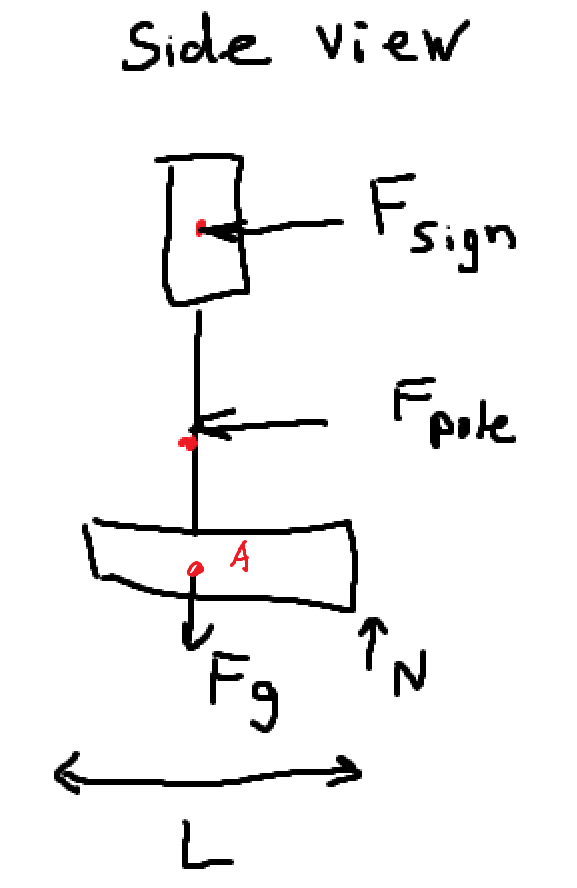
\includegraphics[width=0.5\linewidth]{Questions/Figures/Q3FBD.png}
    \caption{FBD of the concrete block}
    \label{fig:Q3FBD}
\end{figure}

Finding the moment about point $A$,
\begin{align*}
    \sum M_A &= 0 \\
    N (L/2) - 2F_{D,\text{pole}} (2) - F_{D,\text{panel}} (5) &= 0 \\
    g(L W H)\rho (L/2) - 4F_{D,\text{pole}} - 5F_{D,\text{panel}} &= 0 \\
\end{align*}
Solving for $L$,
\begin{align*}
    L &= \sqrt{\frac{10F_{D,\text{panel}} + 8F_{D,\text{pole}}}{g W H \rho}} \\
      &= \sqrt{\frac{10(10.382 \times 10^3) + 8(67.71)}{(9.81)(4)(0.15)(2300)}} \\
      &= \boxed{2.78 \text{ m}}
\end{align*}